\documentclass[../main.tex]{subfiles}
\begin{document}
%\chapter{Theoretical Background}\label{ch:Theory}
\section{Quantum Computing}
Analogous to the digital bits used for classical computation, a quantum computer requires quantum bits, more commonly known as qubits, as the fundamental register. However, unlike the classical bits which can acquire the value of either a 0 or a 1, a qubit state can be a linear superposition of the states $\ket{0}$ and $\ket{1}$, where $\ket{}$ represents a quantum state in the Dirac notation, i.e.,
\begin{equation}
\ket{\psi}= a_0 \ket{0} + a_1 \ket{1},  \label{eq:b1}
\end{equation}
where $a_0$ and $a_1$ are the complex amplitudes such that ${\abs{a_1}}^2 +{\abs{a_0}}^2 =1$. According to the principles of quantum mechanics, a measurement of the qubit state then yields either 0, with probability ${\abs{a_0}}^2$, or 1, with probability ${\abs{a_1}}^2$. 

In its simplest form, a qubit is therefore a two-level system. A spin-$1/2$ particle with its two levels being the up spin and the down spin, can naturally be used as a qubit. In this notation, it is conventional to associate the state $\ket{0}$ with $\ket{\uparrow}$, and the state $\ket{1}$ with $\ket{\downarrow}$. The three components of the Pauli matrices corresponding to the spin-1/2 operator \textbf{S} spanned by these states are:
\begin{center}
$ \sigma_x= \begin{pmatrix}
0 & 1\\
1 & 0
\end{pmatrix}, \sigma_y= \begin{pmatrix}
0 & -i\\
i & 0
\end{pmatrix}, \sigma_z= \begin{pmatrix}
1 & 0\\
0 & -1
\end{pmatrix},
$\\
\end{center}
which are then used as the fundamental elements of quantum computing.\\

For $N$ such qubits, the basis state is a tensor product of the single-qubit basis states. Since each single state requires two basis vectors, the $N$-qubit state comprises of $L=2^N$ basis vectors. This constitutes the computational basis
\{$\ket{00...0}, \ket{00...1},..., \ket{11...1}$\}. Therefore, a general $N$-qubit state can be represented as

\begin{equation}
\ket{\psi} =a_0 \ket{00...0}+a_1 \ket{00...1}+...+a_L \ket{11...1},
\label{eq:b2}
\end{equation}
which requires $L$ complex amplitudes for its description.

The computational basis can be more conveniently notated as $\ket{00...0}=\ket{0}$, $\ket{00..1}=\ket{1}$,..., $\ket{11...1}=\ket{L}$. In this representation, Eq.~(\ref{eq:b2}) thus becomes
\begin{equation}
\ket{\psi}= a_0\ket{0}+a_1\ket{1}+....+a_L\ket{L}.  \label{eq:b3}
\end{equation}
Therefore, the Hilbert space spanned by $N$ qubits is an $L$-dimensional space.

Since Pauli matrices, together with the identity operator I, form a complete basis for the vector space in $2 \times 2$ matrices, any gate acting on a qubit can be expressed as a linear combination of Pauli matrices. The action of a Pauli matrix, $\sigma_\alpha$, where $\alpha \in \{x,y,z\}$ on the $j^{th}$ of the $N$ bits of the basis vector is represented as $\sigma_\alpha^j$. Thus, the Pauli operator $\sigma_\alpha^j$ acting on the general state $\ket{\psi}$, given in Eq.~(\ref{eq:b2}), just acts on the $j^{th}$ bit of the basis vector, altering the coefficients $a_0$, $a_1$,...,$a_L$. The other bits of the basis vector remain unchanged as a result of being acted upon by identity matrices, given as
\begin{center}

 $I=\begin{pmatrix}
1&0\\
0&1
\end{pmatrix}_{i \neq j}
$.\\
\end{center}
\section{Optimization Problems and Quantum Annealing} 
Mathematically, an optimization problem comprises of a cost function, $f_0(\textbf{x})$ involving $N$ variables $x_1$, $x_2$, $x_3$,...,$x_N$, such that $\textbf{x}=(x_1,...,x_N)$. The cost function is subjected to multiple constraints $f_i(x) \leq b_i$. The goal is then to find a solution $\mathbf{x_0}$ that minimises (or maximises) the cost function, while satisfying all the constraints.\\

For satisfiability problems the cost function is written as a Boolean expression in the form of conjunction (a Boolean AND operation) of $r$ clauses, where each clause is a disjunction (a Boolean OR operation) of $k$ variables or their negations ($k$-SAT problems)\cite{boyd2004convex,hsu2018quantum,thomas2014quantum}. A 2-SAT instance is thus formulated as a Boolean expression where each clause is a disjunction of two literals. The literals, $L_{i,j}$, are Boolean variables or their negations. The task is then to find a truth assignment to the Boolean variables that makes the formula $G=(L_{1,1} \lor L_{1,2}) \land (L_{2,1} \lor L_{2,2}) \land ... \land (L_{r,1} \lor L_{r,2})$ true. If $G$=1 then the 2-SAT instance is satisfiable.

Many physically inspired approaches have been adopted to find the solution for the optimization problems. One of the widely used techniques is to encode the problem into the couplings of Ising Hamiltonians \cite{hormozi2017nonstoquastic}. The ground state of this Hamiltonian, corresponding to the state of the minimum energy, then represents the optimal solution of the problem. At low enough temperatures, the system state should eventually relax to the ground state, yielding the required solution.

For finding the optimal solution, the whole spectrum of the Hamiltonian needs to be explored. This requires that the system should be able to escape from a local minimum, if it gets trapped in one, during the course of annealing. The presence of multiple local minima thus makes the determination of the optimal solution harder \cite{santoro2006optimization}.\\
 
The method of simulated annealing was therefore utilised \cite{kirkpatrick1983optimization}, where adding thermal fluctuations to the cost function, keeps the system from getting trapped in the local minima. Yet if the potential barrier becomes very high, this approach may fail. It was in this spirit that the technique of quantum annealing was first employed by B.Apolloni, C.Carvalho and D.de Falco in 1988 \cite{apolloni1989quantum}, wherein quantum fluctuations were used in place of thermal fluctuations. By making use of the quantum tunnelling effect, this approach can still allow for the search of global minima as the system state can tunnel between the local minima \cite{Albash_2018}.\\
 
The cost function is mapped onto the Ising model, making use of the external magnetic field ${h_i}^z$ and the spin couplings ${J_{ij}^z}$ of the model, and thus has the following form:
\begin{equation}
H_P=-\sum\limits_{i=1}\limits^{N}{h_i}^z{\sigma_i}^z - \sum\limits_{\langle i,j \rangle}{J_{ij}^z} {\sigma_i}^z{\sigma_j}^z, \label{eq:b4}
\end{equation}
where ${\sigma_i}^z$ denotes the z component of Pauli-spin matrix acting on the $i^{th}$ spin, and the set $\langle i,j \rangle$ represents the set of pairwise couplings.


The recipe for the annealing algorithm consists of starting with an initial Hamiltonian $H_I$, whose ground state can be easily determined and realised. Most commonly used is the transverse field Hamiltonian: 
\begin{equation}
H_I=-\sum\limits_{i=1}\limits^{N}{h_i}^x{\sigma_i}^x. \label{eq:b5}
\end{equation}
The ground state of $H_I$ is therefore the uniform superposition state: 
\begin{equation}
\ket{\psi}=\frac{1}{{(\sqrt{2})}^N}{(\ket{0}+\ket{1})}_1 \otimes {(\ket{0}+\ket{1})}_2 \otimes....\otimes{(\ket{0}+\ket{1})}_N. \label{eq:b6}
\end{equation}
The Hamiltonian is then slowly swept towards the problem Hamiltonian, with the means of an annealing parameter, say $s$, defined as $s(t)=t/T_A$, where $t$ is the instantaneous time, and $T_A$ is the total annealing time. The Hamiltonian, $H(t)$, corresponding to the most straightforward annealing scheme, is then given by: 
\begin{equation}
H(t)= (1-s(t))H_I + s(t)H_P. \label{eq:b7}
\end{equation}

\begin{comment}
Figure (\ref{fig:b1}) shows the chosen annealing scheme in terms of the annealing parameter.
\begin{figure}[H]
\centering 
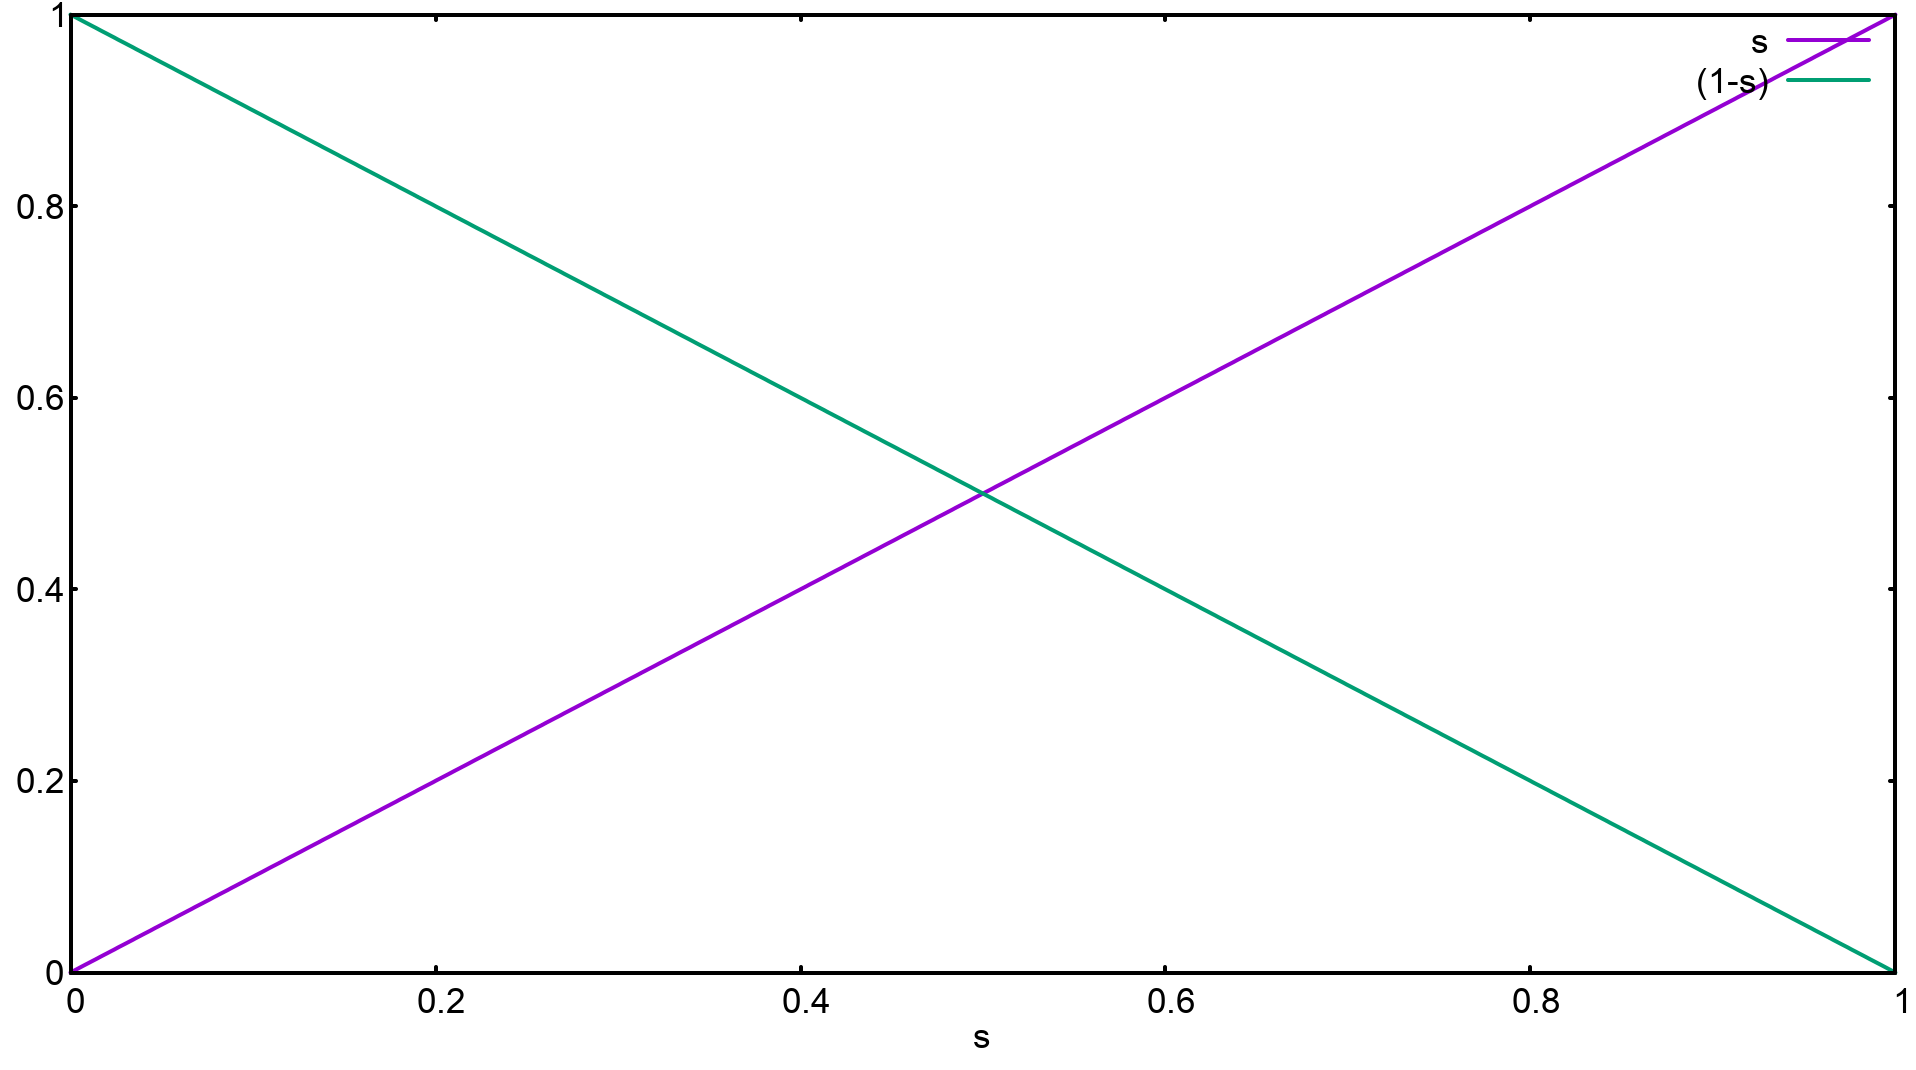
\includegraphics[scale=0.3]{Scheme.png}
\caption{The linear annealing scheme chosen, in terms of the annealing parameter s.}
\label{fig:b1}
\end{figure}
\end{comment}
Therefore, the Hamiltonian transitions from the initial Hamiltonian, $H(t=0)=H_I$ to the final Hamiltonian, $H(t=T_A)=H_P$. \\

According to the \textbf{quantum adiabatic theorem}, the instantaneous state of the system stays close to the ground state of the Hamiltonian $H(t)$, if one starts with the ground state of the initial Hamiltonian and if the driving from the initial Hamiltonian to the problem Hamiltonian is slow enough, which is determined by the minimum energy gap, $\Delta_{min}$, between the ground state and the first excited state of the Hamiltonian $H(t)$ during the course of annealing \cite{born1928beweis,kato1950adiabatic,farhi2000quantum}. Mathematically, adiabatic theorem of evolution holds when 
\begin{equation}
t \gg \max\limits_{0 \leq s \leq 1} \frac{\left| \left| \bra{1(s)}\frac{dH(s)}{ds}\ket{0(s)}\right| \right|}{\Delta_{min}^2}, \label{eq:b8}
\end{equation}
where $\ket{0(s)}$ and $\ket{1(s)}$ represent the instantaneous ground state and the first excited state of the Hamiltonian. Therefore, the performance of quantum annealing depends strongly on the minimum energy gap.\\
Thus, the problem of finding the optimal solution reduces to the problem of solving the time dependent Schr{\"o}dinger equation for the resulting $H(t)$ (see Eq.~\ref{eq:b7}):
\begin{equation}
i\frac{\partial}{\partial t}\ket{\psi}=H(t)\ket{\psi}.    \label{eq:b9}
\end{equation}

However, the process of evolution, starting from the trivial ground state of the initial Hamiltonian and going to a non-trivial ground state of the problem Hamiltonian, may be accompanied by a quantum phase transition. Such a transition is characterized by a vanishing energy gap in the thermodynamic limit. For the problems which are considered to be difficult, the minimum gap is found to close exponentially as a function of the system size, i.e., $\Delta_{min} \propto e^{-cN}$, for a positive constant $c$ and $N$ number of spins. This suggests that the annealing time required to ascertain that the evolution is adiabatic also grows exponentially, $T_A \propto e^{2cN}$. On the other hand, if the gap closes polynomially ($\Delta_{min} \propto N^{-l}$, for a positive constant $l$), the computation time is also polynomial, $T_A \propto N^{2l+1}$, and the problem is considered easy \cite{hauke2019perspectives}.

Therefore, the dependence of the minimum energy gap on the size of the system determines the annealing time required to make the evolution of the state of the system to be adiabatic. Thus, one method of improving the performance of quantum annealers is by controlling the closing of the gap. Altering the annealing scheme is believed to be one of the ways by which this can be achieved \cite{Albash_2018,hauke2019perspectives,farhi2002quantum,crosson2014different,hormozi2017nonstoquastic}. In this work we aim to achieve the same by including a third Hamiltonian, a trigger Hamiltonian - $H_T$ in the time dependent Hamiltonian $H(t)$ (see Eq.~\ref{eq:b7})\cite{Albash_2018,farhi2002quantum,crosson2014different,hormozi2017nonstoquastic}. The trigger Hamiltonian should vanish at both the start and end of the annealing process, so that one can still start with the easily realizable ground state of the initial Hamiltonian, and the resulting state of the problem Hamiltonian remains unaffected. The Hamiltonian thus takes the form: 
\begin{equation}
H(t)= (1-s(t))H_I + g s(t)(1-s(t))H_T + s(t)H_P ,\label{eq:b12}
\end{equation} 
where parameter $g$ controls the strength of the added trigger.\\

In this thesis we deal with two types of trigger Hamiltonians - a ferromagnetic trigger (F) and an anti-ferromagnetic trigger (A)\cite{hormozi2017nonstoquastic}, defined as
\begin{equation}
H_T^F = - \sum\limits_{\langle i,j\rangle}{\sigma_i}^x{\sigma_j}^x,    \label{eq:b13}
\end{equation}
and
\begin{equation}
H_T^A= +\sum\limits_{\langle i,j \rangle}{\sigma_i}^x{\sigma_j}^x,          \label{eq:b14}
\end{equation}
with the same pairwise coupling set $\langle i,j \rangle$ as for the problem Hamiltonian. Equivalently, the trigger can also be chosen to have the form $\pm {\textstyle\sum}_{\langle i,j\rangle}{\sigma_i}^y{\sigma_j}^y$.
As will be seen in the following chapters, adding these triggers alters the energy spectrum considerably, which in turn affects the overlap of the final state with the ground state in different ways. \\


The following sections focus on two approaches that have been used in this work to solve the time-dependent Schr{\"o}dinger equation. The Suzuki-Trotter product formula has been adopted to track the evolution of the state, and to compute the overlap of the final state with the already determined ground state of the problem Hamiltonian. The full diagonalization method, on the other hand, has been used to calculate the errors involved in using the Suzuki-Trotter approximation, and to determine the energy spectra and minimum gaps for $H(t)$ for $t \in [0,T_A]$, where $T_A$ is the total annealing time.

\section{Exact Diagonalization}
This method consists of determining the eigenvalues and eigenvectors of the Hamiltonian matrix, which is an $L\times L$ ($2^N \times 2^N$) matrix, at each time step.

For constructing the Hamiltonian matrix at time step $t$ $\in [0,T_A]$, all the basis vectors in the computational basis are acted upon by the instantaneous Hamiltonian, given by Eq.~(\ref{eq:b12}). The action of the Hamiltonian on the $i^{th}$ basis vector corresponds to the $i^{th}$ column of the Hamiltonian matrix, e.g. for $\ket{\psi}=(1,0,...,0)^T$, $H\ket{\psi}$ gives the first column of the Hamiltonian matrix. \\
The resulting matrix is then diagonalized to obtain the eigenvalues $\Lambda$, and unitary matrix of the eigenvectors, V. Since $V^{\dagger}HV=\Lambda$, the unitary evolution operator $U(t)=e^{-itH}=Ve^{-it\Lambda}V^{\dagger}$.


This approach, however, has some serious limitations. First, the memory requirement to store the Hamiltonian matrix grows as $\mathcal{O}(2^{2N})$ with the number of qubits $N$. Additionally, full diagonalization takes $\mathcal{O}(2^{3N})$ floating-point operations \cite{de2004computational}. Therefore, this method is rendered impractical for solving the time dependent Schr{\"o}dinger equation for systems more than 20 qubits.

\section{Suzuki-Trotter Product Formula} 
For solving the TDSE (see Eq.~\ref{eq:b9}), one needs to evaluate the unitary matrix exponentials of the evolution operator, $U(t)$ given as:
\begin{equation}
U(t)= e^{-itH}= e^{-it(H_1+...+H_K)}= \lim\limits_{m \to \infty} {\bigg(\prod_{k=1}^{K}e^{-itH_k/m} \bigg)}^m.    \label{eq:b15}
\end{equation}
In this work, the Lie-Trotter-Suzuki product formula \cite{de2004computational,trotter1959product,suzuki1977monte} is employed to construct unitary approximations to the evolution operator. Defining $\tau$ as $t/m$, to be the time step at which the evolution operator is applied, a repeated application of $U(\tau)$ yields $U(t)$. For a sufficiently small time step $\tau$, the first order approximation for $U(t)$ in Eq.~(\ref{eq:b15}) is
\begin{equation}
\tilde{U}_1(\tau)=e^{-i\tau H_1}...e^{-i\tau H_K},    \label{eq:b16}
\end{equation}
which holds good if $\tau \left| \left| H_i \right| \right| \ll 1$ for all $i$=1,..,$K$.

For an improved accuracy, a second order approximation is made to $U(t)$ in Eq.~(\ref{eq:b15}), using $\tilde{U}_1(\tau)$ from Eq.~(\ref{eq:b16}):
\begin{equation}
\tilde{U}_2(\tau)=\tilde{U_1}^{\dagger}(-\tau/2)\tilde{U_1}(\tau /2)=e^{-i\tau H_K/2}...e^{-i\tau H_1/2}e^{-i\tau H_1/2}...e^{-i\tau H_K/2}.
\end{equation}
Since $\tilde{U}_1(\tau)$ is unitary, as all $H_k$ in Eq.~(\ref{eq:b15}) are Hermitian, $\tilde{U}_2(\tau)$ is also unitary. The measure of error, calculated using the 2-norm of the difference between $U(\tau)$ and  $\tilde{U}_2(\tau)$, grows cubically in $\tau$ \cite{de2004computational,de1989simulation,de1987product}, i.e.
\begin{equation}
\left| \left| U(\tau)-\tilde{U}_2(\tau) \right| \right| \leq c\tau ^3    
\end{equation} 
for a positive constant $c$. Since the whole annealing process requires $m$ such time steps, the involved error becomes
\begin{equation}
\left| \left| U(t)-\tilde{U}_2(m \tau) \right| \right| \leq m c \tau^3.  \label{eq:b17}
\end{equation}
Since $m \tau=t$, (\ref{eq:b17}) is equivalent to
\begin{equation}
\left| \left| U(t)-\tilde{U}_2(m \tau) \right| \right| \leq ct\tau^2. \label{eq:b18}
\end{equation}


\begin{comment}
Substituting (\ref{eq:b5}),(\ref{eq:b13} or \ref{eq:b14}) and (\ref{eq:b4}) in (\ref{eq:b12}), we obtain:
\begin{equation}
H(t)=(1-s)\Big(-\sum \limits_{i=1}\limits^N h_i^x \sigma_i^x \Big)+g*s(1-s)\Big(\mp \sum \limits_{<i,j>}\sigma_{j}^x\Big) +s \Big(-\sum\limits_{i=1}\limits^{N}{h_i}^z{\sigma_i}^z - \sum\limits_{<i,j>}{J_{ij}^z} {\sigma_i}^z{\sigma_j}^z \Big).  \label{eq:b19}
\end{equation}
\end{comment}


The Hamiltonian H(t) is then decomposed as follows:
\begin{equation}
H=H_{single}+H_x+H_Y+H_z, \label{eq:b20}
\end{equation}
where $H_{single}=-(1-s){\textstyle\sum}_{i=1}^{N}({h_i}^x{\sigma_i}^x )-s({\textstyle\sum}_{i=1}^{N}{\sigma_i}^z)$, $H_x= \mp (1-s) ( {\textstyle\sum}_{\langle i,j\rangle}{\sigma_i}^x{\sigma_j}^x)$, $H_y= \mp (1-s) ({\textstyle\sum}_{\langle i,j\rangle}{\sigma_i}^y{\sigma_j}^y)$, and $H_z= -s ({\textstyle\sum}_{\langle i,j\rangle}{\sigma_i}^z{\sigma_j}^z )$. In general, we have
\begin{equation}
e^{i \mathbf{v.\sigma}}=cos(v) I +i \frac{sin(v)}{v}\mathbf{v.\sigma},
\end{equation}
where I represents the identity matrix, and $v=\sqrt{v_x^2 +v_y^2 +v_Z^2}$. Then, 
\begin{equation}
e^{-itH_{single}}=\prod \limits_{i=1} \limits^{N} e^{it[(1-s)\sum \limits_i h_i^x \sigma_i^x +s \sum \limits_{i} h_i^z \sigma_i^z]} = \prod \limits_{i=1} \limits^{N} \begin{pmatrix}
\cos(th_i) +i \frac{sh_i^z}{h_i} \sin(th_i) &  i \frac{(1-s)h_i^x}{h_i} \sin(th_i)\\
i \frac{(1-s)h_i^x}{h_i}\sin(th_i) & \cos(th_i) -i \frac{sh_i^z}{h_i} \sin(th_i),
\end{pmatrix}
\end{equation}
where $h_i=\sqrt{(1-s(t))^2 {h_i^x}^2 + s(t)^2 {h_i^z}^2}$.\\

The computational basis states are the eigenstates of the Pauli-z operator, $\sigma^i_z$. Thus $e^{-itH_z}$ is a diagonal matrix in the computational basis, and its action on the input state changes the phase of each of the basis vectors. As $H_z$ is a sum of pair interactions, it is trivial to implement this operation \cite{de2004computational}.\\

The same approach can be adopted for implementing $H_x$ operations as well, by using the rotation operators $Y_j$ as follows. Writing $Y={\textstyle\prod}_{i=1}^{N} Y_i$, we obtain
\begin{equation}
e^{-itH^x}=\bar{Y}Y e^{-itH^x}\bar{Y}Y=\bar{Y}e^{it \sum \limits_{\langle i,j \rangle} J_{ij}^x \sigma_i^z \sigma_j^z} Y.
\end{equation}
This completes the specifications required to solve the TDSE.

\end{document}